\section{Step 1 - The frame}
Our first step is to provide a frame which is used in the next steps.
Read and run {\tt Step1.py} (see listing~\ref{LISTING_STEP1_PY} given below)
\footnote{In the following sections only the relevant parts of the code is presented in the script.
If you are not sure how this code fits into the program please use the example code.}.

Figure~\ref{STEP_1_SCREEN} shows what you should get if you execute {\tt Step1.py}.
If you installed all what's needed you should see our empty pythonOCC screen.
Please study the code and the comments added.
If you have questions concerning all the wxPython stuff don't worry.
The comments in the code provide more information than needed for following this step by step course.
If you just accept the code as it is and try to figure out how to get something similar done that's fine for the moment.
If you want to have a closer look I recommend the book of Noel Rappin and Robin Dunn~\cite{WXPYTHON_IN_ACTION}.
% +++++++++++++++++++++++++++++++++++++++++++++++++++++++++++++++++++++++ 
% +++ Bild: Step 1 ++++++++++++++++++++++++++++++++++++++++++++++++++++++
% +++++++++++++++++++++++++++++++++++++++++++++++++++++++++++++++++++++++ 
\begin{figure}[h]
\begin{center}
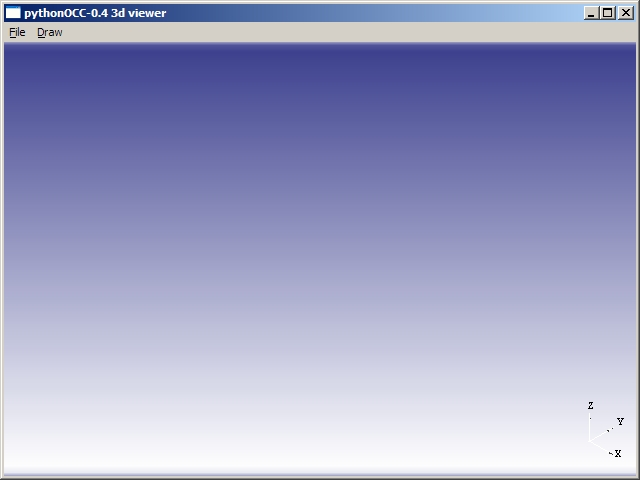
\includegraphics[height=8.5cm,width=11.3cm]{Step1.jpg}
\end{center}
\caption[Screenshot of Step1]{\label{STEP_1_SCREEN}Screenshot of Step1}
\end{figure}

\begin{python}[moreemph={[4], 46, 48},caption={Step1.py - The program frame},label=LISTING_STEP1_PY]
# =============================================================================
# Packages to import
# =============================================================================
import wx
import sys

from OCC import VERSION
from OCC.Display.wxDisplay import wxViewer3d

# =============================================================================
# Functions called from some menu-items
# =============================================================================
def draw_nothing(event=None):
    pass

def exit(event=None):
    sys.exit()

# =============================================================================
# This is the Application Frame class for wx
# =============================================================================
class AppFrame(wx.Frame):
    def __init__(self, parent):
        wx.Frame.__init__(self, 
                          parent, 
                          -1, 
                        "pythonOCC-%s 3d viewer"%VERSION, 
                        style=wx.DEFAULT_FRAME_STYLE,
                        size = (640,480))
        self.canva = wxViewer3d(self)      
        self.menuBar = wx.MenuBar()
        self._menus = {}
        self._menu_methods = {}
    
    # Function for creating new menus like File, Edit, View, and so on
    # The stuff appearing at the top    
    def add_menu(self, menu_name):
        _menu = wx.Menu()
        self.menuBar.Append(_menu, "&"+menu_name)
        self.SetMenuBar(self.menuBar)
        self._menus[menu_name]=_menu

    # Function for creating new menu items like File-New, File-Exit, Edit-Copy, 
    # Edit-Cut, Edit-paste, and so on
    # The stuff appearing if a menu is selected
    def add_function_to_menu(self, menu_name, _callable):
        _id = wx.NewId()
        assert callable(_callable), 'the function supplied isnt callable'
        try:
            self._menus[menu_name].Append( \
                        _id, 
                        _callable.__name__.replace('_', ' ').lower() )
        except KeyError:
            raise ValueError, 'the menu item %s doesnt exist' % (menu_name) 
        self.Bind(wx.EVT_MENU, _callable, id=_id)


# =============================================================================
# Called from Main-part. Calls itself frame methods.
# =============================================================================
def add_menu(*args, **kwargs):
    frame.add_menu(*args, **kwargs)
    
def add_function_to_menu(*args, **kwargs):
    frame.add_function_to_menu(*args, **kwargs)

def start_display():    
    '''
    call the mainloop
    '''
    global app
    app.MainLoop()
    
# =============================================================================
# Main-part
# If this script is running as a main script, i.e. it is directly called
# by Python the following is executed.
# =============================================================================
if __name__ == '__main__':
    # Create Application - with wx.PySimpleApp() we do not need an OnInit
    app = wx.PySimpleApp()
    wx.InitAllImageHandlers()
    # Create Application Frame
    frame = AppFrame(None)
    frame.Show(True)
    wx.SafeYield()
    frame.canva.InitDriver()
    app.SetTopWindow(frame)
    display = frame.canva._display
    # Show a background image
    display.SetBackgroundImage("bg.bmp")  
    # This is the place where we hook our functionality to menus
    # ----------------------------------------------------------
    add_menu('File')
    add_function_to_menu('File',  exit)
    add_menu('Draw')
    add_function_to_menu('Draw', draw_nothing)
    
    start_display()
\end{python}


That's the frame so get ready to add some geometry.
